%\documentclass[10pt,twocolumn]{main}
%\documentclass[10pt,letterpaper]{article}
\documentclass[conference]{IEEEtran}

%next line allows \thanks in conference mode
\IEEEoverridecommandlockouts

\usepackage{pslatex}
\usepackage{amsmath}
\usepackage{amssymb}
%\usepackage{graphics}
%\usepackage{epsfig} % for postscript graphics files

\DeclareMathOperator{\Drift}{Drift}

\usepackage{cite}
\ifCLASSINFOpdf
  \usepackage[pdftex]{graphicx}
  % declare the path(s) where your graphic files are
  % \graphicspath{{../pdf/}{../jpeg/}}
  % and their extensions so you won't have to specify these with
  % every instance of \includegraphics
  \DeclareGraphicsExtensions{.pdf,.jpeg,.png}
\else
  % or other class option (dvipsone, dvipdf, if not using dvips). graphicx
  % will default to the driver specified in the system graphics.cfg if no
  % driver is specified.
  \usepackage[dvips]{graphicx}
  % declare the path(s) where your graphic files are
  % \graphicspath{{../eps/}}
  % and their extensions so you won't have to specify these with
  % every instance of \includegraphics
  \DeclareGraphicsExtensions{.eps}
\fi


\begin{document}

\title{On the Impact of Time Synchronization on Quality of Information and Network Performance
\thanks{This material is supported in part by the U.S. ARL and the
U.K. MOD under Agreement Number W911NF-06-3-0001, by the NSF under
award CNS-0614853, and by the Center for Embedded Networked Sensing
at UCLA. Any opinions, findings and conclusions or recommendations
expressed in this material are those of the authors and do not
necessarily reflect the views of the listed funding agencies. The
U.S. and U.K. Governments are authorized to reproduce and distribute
reprints for Government purposes notwithstanding any copyright
notation herein.}}
\author{{\sc Kartik Ariyur\dag}, {\sc Thomas Schmid\ddag}, {\sc Yunjung Yi\dag}, {\sc Zainul Charbiwala\ddag}, {\sc Mani B. Srivastava\ddag}\\
\normalsize{\dag Honeywell Inc.} \\
\normalsize{1985 Douglas Drive Golden Valley, MN}\\
\normalsize{\tt\{kartik.ariyur,yunjung.yi\}@honeywell.com}\\
\normalsize{\ddag Department of Electrical Engineering, }
\normalsize{University of California, Los Angeles} \\
\normalsize{420 Westwood Plaza Los Angeles, CA}\\
\normalsize{\tt\{thomas.schmid,zainul,mbs\}@ucla.edu} }

\maketitle
%\setcounter{page}{0}
%\pagestyle{empty}
\newtheorem{theorem}{Theorem}
\newtheorem{assumption}{Assumption}
\baselineskip=1.\normalbaselineskip
\begin{abstract}

New hardware and technologies enable low-power low-cost distributed
sensing systems. To realize certain applications such as real-time event
detection, target tracking, and system monitoring, time synchronization is
essential. However, time synchronization both consumes limited battery power on the network nodes and can clog the bandwidth of the network. The choice of a time synchronization mechanism will depend on the
application's requirement of timing accuracy as well as its energy budget. We derive the effect of time synchronization accuracy upon real time estimation and detection problems. We also quantify the costs and benefits of time synchronization algorithms. The intuitive assumption that using higher stability clocks will
automatically improve duty cycling performance, and thus decrease power
consumption, does not always hold true. In this article, we present the
link between clock stability, impact on duty cycling, and the possible bandwidth
savings that can be achieved by using temperature compensated clocks or clock drift
estimation techniques. This paper formalizes this relationship based on an analytical framework using representative applications, namely, event detection and estimation. The analysis shows the impact of timing errors for different event durations, target
speeds, number of sensors, and sampling frequencies. The analysis
framework can also be used to estimate the maximum synchronization error
each application can sustain while still achieving the desired Quality of Information (QoI).  
\end{abstract}

\section{Introduction}
New hardware and technology enable low-power inexpensive
distributed sensor networks. To realize certain applications such as
real time event detection, target tracking and system monitoring,
time synchronization is essential. There exists substantial literature on 
synchronization techniques including Time-Sync
Protocol for Sensor Network (TPSN)~\cite{ganeriwal03timingsync},
Reference Broadcast Synchronization (RBS)
~\cite{elson02finegrained}, elapsed time \cite{kusy05elapsed}, and Flooding Time Synchronization Protocol (FTSP)~\cite{maroti2004ftsp}.
In general, the goal of a time synchronization mechanism is to
devise a scheme that improves accuracy with minimal energy
consumption. However, there is clearly a trade off between accuracy and
energy consumption. It is not always be desirable to deploy the
most accurate time synchronization as it can prematurely drain the batteries. The
choice of a time synchronization mechanism will depend on the
application's demand on timing accuracy as well as the available energy
budget. To select a proper time
synchronization mechanism based on the requirements of the application, the relationship between application
performance or QoI (Quality of Information) and time synchronization
services are quantified in this article. We
formalize the relationship between the performance of applications
and time synchronization services based on an analytic framework using
representative applications, namely, event detection and estimation.

The paper is organized as follows. Section~\ref{sec:detector} quantifies the effect of the time-error between nodes upon the performance of detection algorithms, both for the case of no synchronization algorithm and for the case where synchronization algorithms are used. Section~\ref{sec:TrackingFilter} introduces a novel nonlinear hybrid filter which is globally convergent and robust to synchronization errors. It also quantifies the effect of synchronization error upon the solution of least squares estimation problems across the network, which would automatically include batch least squares, recursive least squares and Kalman filtering. Section~\ref{sec:power} quantifies the trade-off between clock stabilization, power consumption, and synchronization across the network. In particular, it shows how much energy a duty-cycled system can gain by employing
a more stable clock, and conversely, it shows the maximum energy such a
clock system can use so that overall energy consumption is minimized. Upper and lower bounds on the number of resynchronization requests are determined using a 3 year temperature data set and modeling crystal drifts.



%\section{Introduction}
New hardware and technology enable low-power inexpensive
distributed sensor networks. To realize certain applications such as
real time event detection, target tracking and system monitoring,
time synchronization is essential. There exists substantial literature on 
synchronization techniques including Time-Sync
Protocol for Sensor Network (TPSN)~\cite{ganeriwal03timingsync},
Reference Broadcast Synchronization (RBS)
~\cite{elson02finegrained}, elapsed time \cite{kusy05elapsed}, and Flooding Time Synchronization Protocol (FTSP)~\cite{maroti2004ftsp}.
In general, the goal of a time synchronization mechanism is to
devise a scheme that improves accuracy with minimal energy
consumption. However, there is clearly a trade off between accuracy and
energy consumption. It is not always be desirable to deploy the
most accurate time synchronization as it can prematurely drain the batteries. The
choice of a time synchronization mechanism will depend on the
application's demand on timing accuracy as well as the available energy
budget. To select a proper time
synchronization mechanism based on the requirements of the application, the relationship between application
performance or QoI (Quality of Information) and time synchronization
services are quantified in this article. We
formalize the relationship between the performance of applications
and time synchronization services based on an analytic framework using
representative applications, namely, event detection and estimation.

The paper is organized as follows. Section~\ref{sec:detector} quantifies the effect of the time-error between nodes upon the performance of detection algorithms, both for the case of no synchronization algorithm and for the case where synchronization algorithms are used. Section~\ref{sec:TrackingFilter} introduces a novel nonlinear hybrid filter which is globally convergent and robust to synchronization errors. It also quantifies the effect of synchronization error upon the solution of least squares estimation problems across the network, which would automatically include batch least squares, recursive least squares and Kalman filtering. Section~\ref{sec:power} quantifies the trade-off between clock stabilization, power consumption, and synchronization across the network. In particular, it shows how much energy a duty-cycled system can gain by employing
a more stable clock, and conversely, it shows the maximum energy such a
clock system can use so that overall energy consumption is minimized. Upper and lower bounds on the number of resynchronization requests are determined using a 3 year temperature data set and modeling crystal drifts.



%\section{Related Work}

Time synchronization techniques -- RBS, TPSN, Tiny-sync, mini-sync,
elapsed time,

%\section{Application QoI and Time Synchronization}

\subsection{Background}
 Questions that we like to answer
through this analysis includes the followings. 1.  What will happen
if timing errors are not bounded - a sample may have very inaccurate
timing value - can we detect this unusual event (or fault)?

2.  What could be the upper bound of timing error versus sample rate
for estimation application - Is there any relationship between
sample rate and timing error (such as if timing errors are high, do
we need more frequent samples?)

3.  Can we do some fault detection and correction. Such as
maintaining history of samples from each sensor, we can detect some
abnormal behaviors/samples? Or among samples from sensors at certain
duration, we can do also some filtering? 4.  If we want to do this
kind of filtering, do we need better time-sync accuracy?

5.  Does the error characteristic known to the filter help the
accuracy of filtering? Let's say, we can provide a fairly accurate
error model, can filter achieve highly accurate tracking?

\subsubsection{Time synchronization error}
 In our paper, we assume that
a sensor is equipped with an internal hardware oscillator that
provides vibration frequency to keep the local clock continuously
running. The vibration frequency will depend on the size, thickness
and cutting edge of a crystal inside the oscillator and the
condition of sensor's surrounding physical environment.

Generally speaking, we have two sources of synchronization errors
for distributed algorithms: (1) local time change due to clock
drift; (2) message delay uncertainty. These two error sources will
differently impact on the synchronization error depending on
the synchronization technique \cite{wsn-timecali}.

Considering a single node, the local clock of a sensor 'X' at
Coordinated Universal Time (UTC) $t$ can be represented as
\cite{timing-error}
\[t_x = a_xt+ t_{0x} + \Drift_x(t),\]
where $a_x$ is the clock skew, i.e., difference between X's oscillator
and the ideal perfect one, and $t_{0x}$ is the initial time offset.
$\Drift_x(t)$ is the clock drift at time $t$. Clock drift changes with
environment. It is an environment-dependent phenomenon and hard to
be modeled accurately. More detailed discussion on clock drift will
be shown in Section \ref{}.

If we consider two nodes, then we also consider message latency and
other communication-related delay. It can be classified as the
followings further \cite{timing-error}.
\begin{itemize}
\item {\bf P}rocessing delay: the time spent at node S (sender) to
prepare and process the packet, and transfer it to the networking
component.
\item {\bf A}ccess delay: the delay to acquire the wireless medium
\item {\bf P}ropagation delay: the delay to transmit the propagate over
the medium
\item {\bf R}eceive delay: time for the node R (receiver) to
process the packet and get the reading of its local clock
\end{itemize}

In total, the delay to include all the communication can be
represented as $PAPR_{StoR}$, and the time of R relative to S can be
shown as $t_r$ = $a_{rs}(n)t_s$ + $t_{0rs}(n)$ + $PAPR_{StoR}$ ,$nT$
$<$ $t$ $<$ $(n+1)T$, where $T$ is the sampling rate, and $a_{rs}$
is the offset difference between R and S. Detailed information can
be found in ~\cite{timing-error}.

Based on this representation, \cite{timing-error} derives the
limitation on errors between any networked two nodes in terms of
value and distribution. The paper showed that the distribution of
limitation of errors is uniform if communication-related delay is
uniformly bounded. The results from the paper are used in our
analysis.

\subsection{Analysis Framework}
\subsubsection{Event Detection Application}
Section 2.2.1.1 Event detection framework Section \\
2.2.1.2 Analysis on performance of event detection versus various
timing error models Section \\
2.2.2 Target Estimation Application Section \\
2.2.2.1 Target Estimation Filtering Algorithm Section \\
2.2.2.2 Analysis on performance of target estimation versus various
timing error models Section

\subsection{Discussion on relationship between time synchronization service and application
QoI}

%detector
\section{A Simple Probabilistic Detector}\label{sec:detector}
Consider a system of $N$ sensors that are identical and detect an
event of time period $\tau$ such as a gunshot or an explosion. Let
the probability that an event $E$ has occurred, given that the
sensor measurement $s_i$ exceeds a threshold $T$ be given as:
\begin{equation}
P(E|s_i>T)=p \quad \forall i\label{eqn:detrate},
\end{equation}
where $i=1\ldots N$ goes over all the sensors, and $0<p\leq 1$.
Similarly, let the probability of threshold crossing when the
event has not occurred, $E^c$ be given as:
\begin{equation}
P(E^c|s_i>T)=q \forall i\label{eqn:fprate},
\end{equation}
and $0<q\leq 1$. Let the number of samples produced by a sensor in
the course of the event equal $M=\lfloor \tau f_s \rfloor$, where
$f_s$ is the sampling frequency of all the sensors. Considering
the probabilities identical for all of the sensors is realistic if
the sensors respond to low frequency acoustics or thermal
radiation signature, which does not attenuate very much with
distance. Furthermore, we can also assume that the detection is at
the same instant for all of the sensors if the sensors are not
separated by distances larger than the signal would travel in a
sampling interval (e.g., for an acoustic sensor system $10$ms or
$100$Hz sampling gives around $3$ meters separation for the
sensors).

Now consider a detection function defined as follows that combines
data from all of the sensors to detect an event and determine its
time:
\begin{eqnarray}
% \nonumber to remove numbering (before each equation)
  f &=& {1\over MN}\sum_{i=1}^{MN}d_i\label{eqn:detector} \\
  d_i &=&\left\{\begin{array}{lr}
  1 & s_i>T\\
  0 & {\rm otherwise}\end{array}\right.
\end{eqnarray}

The relevant questions that can be asked at this point are--
\begin{itemize}
\item What is the expected value of $f$ if an event occurs? \item
What is the expected value of $f$ if the event does not occur?
\end{itemize}
If there are no bandwidth limitations and there is perfect time
synchronization between the sensors, we will have
\begin{eqnarray}
% \nonumber to remove numbering (before each equation)
  E\langle f|E\rangle &=& p \nonumber\\
E\langle f|E^c\rangle   &=& q\label{eqn:perfectsync}.
\end{eqnarray}
The detection rate will be smaller and the false positive rate will be higher if there are bandwidth limits
and synchronization is not perfect if we threshold the detection function $f$ at the value $p$.

\subsection{Detection Rate under Synchronization Error}
Let us consider the detection system when the different sensors have different detection probabilities $p_i$ and different false positive probabilities $q_i$. The detection function can be expressed as
\begin{eqnarray}
% \nonumber to remove numbering (before each equation)
  f &=& {1\over N}\sum_{i=1}^Md_i \nonumber\\
  d_i &=& {1\over M}\sum_{k=1}^Md_{i,k}\label{eqn:heterog_detector}\\
  d_{i,k}&=& \left\{\begin{array}{lr}
  1 & s_{i,k}>T_i\\
  0 & {\rm otherwise}\end{array}\right.\nonumber
\end{eqnarray}
We can set thresholds using standard Bayesian methods if we know the distributions of noise in the different sensors along with the signal levels produced by the events. To consider the effect of synchronization error on the detector, let us assume that it follows a uniform distribution over the interval $[0,\epsilon]$ or almost equivalently, $[0,L]$, where $L=\lfloor \epsilon f_s\rfloor$, and that this distribution is identical for all the sensors. We assume here that $\epsilon$ is the maximum that clocks on any two network nodes drift away from each other, either during sleep or for the time of operation of the network. Now the probability that the sample of length $MN$ from which $f$ is computed was not produced in the interval $[t-\tau,t]$, or in the sampled case, $[k-M,k]$ can be calculated. We examine the most probable case that the event occurs in the interval $[k-M,k]$, and there is no event in the preceding interval. We assume that all detection results from individual sensors are transmitted to the node which produces $f$--we later generalize to the case where some of the bits are lost in transmission. Consider a sample received at time $l$ in the interval $[k-M,k]$. The probability that it came from a sensor before the event started is
\begin{equation}
% \nonumber to remove numbering (before each equation)
  p_{se,l} = \left\{\begin{array}{lr}
  {L-(l-k+M) \over L}  & L-M+k-l\geq 0\\
  0 & {\rm otherwise}\end{array}\right.\label{eqn:syncerrorprob},
\end{equation}
and the probability that it came from during the event is $1-p_{se,l}$. Without loss of generality, we can take $k=M$ or any multiple of it, so that $l$ goes from $0$ to $M$. Hence, the expected value of the composite detector $f$ can be calculated from the individual values of the $d_{i,l}$ as follows:
\begin{eqnarray}
% \nonumber to remove numbering (before each equation)
  E\langle f\rangle &=& {1\over N}\sum_{i=1}^N\langle d_i \rangle\nonumber\\
  E\langle d_i \rangle&=& {1\over M}\sum_{l=1}^M p_i(1-p_{se,l})+q_ip_{se,l}\nonumber\\
  &=& p_i\left( {M+1 \over 2L}\right)+q_i\left(1- {M+1 \over 2L}\right)\label{eqn:heterog_detector_mean}
\end{eqnarray}
We can use these calculations in conjunction with the distributions
in~\cite{timing-error} to obtain realistic detector performance
shown in Section \ref{sec:tighter_analysis}.

Figure \ref{fig:detection} shows the detection probability $E\langle
f\rangle$ with time synchronization error bound of 1ms and 1s drawn
in solid and dotted line respectively. Here, we assume that $p_i$ =
0.9 and $q_i$ = 0.05 with 10 randomly deployed sensors. The event
duration is 1 second for the analysis. In the figure, we can observe
two important results. First, the impact of timing error on
detection probability is significant. If the timing error is bounded
within 1 second, the detection probability is considerably lowered
compared to the case where timing error is bounded within 1ms. Thus,
reasonable timing error bounds are mandatory to achieve a good QoI.
Secondly, the application QoI is not linearly improved with sampling
rate. It shows a tendency that the detection probability is slightly
impaired with 2 $\sim$ 5 samples in the event duration period (0.5
$\sim$ 0.2 sampling frequency with 1 second event duration).
Opposite to our intuition that the detection probability would be
improved as the sampling rate increases, the sampling rate or
sampling frequency has minimal impact on detection application's
QoI. Rather, the limit of timing error plays more critical role in
terms of QoI.

\begin{figure}
    \begin{center}

    \includegraphics[height=0.3\textheight,width=0.45\textwidth,bbllx=49,bblly=101,bburx=585,bbury=714]{figures/detectionfig}
    \caption{Detection Probability with various sampling frequencies}
        \label{fig:detection}
    \end{center}
\end{figure}
\subsection{Dependence of Detection upon Synchronization Error: A More Precise
Analysis}\label{sec:tighter_analysis} The preceding analysis of the
dependence of detection accuracy on synchronization error assumes
there is no actual synchronization process going on--that the
sensors are just left unsynchronized and the clocks drift from each
other within a certain bound. This gives conservative results
compared to a scheme where there is some synchronization and the
error distribution is not uniform but rather, bell shaped. There are
two reasons for this--when no time stamps are passed around,
measurements that arrive can be simply be taken to be from the past.
But when there is a synchronization algorithm that is attempting to
synchronize all the clocks, we get measurements with time stamps and
we have to concern ourselves with the error in the time stamp to
determine detector performance.

A distribution of the time error between two networked nodes, combining process delay, access delay, propagation delay, and receive delay is developed in~\cite{timing-error}. Assuming a uniform distribution of this error, they show that a maximum absolute error of $b>0$ in the time error results in a maximum synchronization error of $3b$ and a probability distribution of synchronization error over the interval $[-3b, 3b]$ as follows:
\begin{equation}\label{eqn:syncerrordist}
    f_s^b(t)=\left\{\begin{array}{lr}
    {9 \over 8 b}-{9 \over 8 b^2}t+{3\over8 b^3}t^2-{1\over 24b^4}t^3, & 2b<t<3b\\
    {11\over 24b}-{1\over 8b^2}t-{1\over 8b^3}t^2+{1\over 24b^4}t^3, & b<t<2b\\
    {5\over 12b}-{1\over 4b^3}t^2+{1\over 12 b^4}t^3, & 0<t<b\\
    {5\over 12b}-{1\over 4b^3}t^2-{1\over 12 b^4}t^3, & -b<t<0\\
    {11\over 24b}+{1\over 8b^2}t-{1\over 8b^3}t^2-{1\over 24b^4}t^3, & -2b<t<-b\\
    {9 \over 8 b}+{9 \over 8 b^2}t+{3\over8 b^3}t^2+{1\over 24b^4}t^3, & -3b<t<-2b\\
    0, &\mathrm{otherwise.}
    \end{array} \right.
\end{equation}
The question we answer with this probability distribution is--what is the probability $p_{in,i}$ that a measurement time stamped as being in an interval came from within it? The answer is obtained through integrating $f_s^b(t)$ from $-t_i$ to $\tau-t_i$ where the duration of the event is $\tau$ and $t_i$ is the time already elapsed during the event. The probability that it didn't come from within the interval is simply $p_{out,i}=1-p_{in,i}$
\begin{equation}
p_{in,i}=\int_{-t_i}^{\tau-t_i}f_s^b(t)dt\label{eqn:pin} .
\end{equation}
To write the expression for $p_{in,i}$ in a compact form, we first create the notation needed for the integrals of the the probability distribution over the different intervals--we denote them in terms of the interval of integration and the time to which the integration is performed $c_{[a b],t}$denotes the integral of the pdf within the interval to the point $t$.
\begin{eqnarray}
% \nonumber to remove numbering (before each equation)
c_{[2b, 3b],t} &=&      {9 \over 8 b}(t-2b)-{9 \over 16 b^2}(t^2-4b^2)\nonumber\\
&&+{1\over8 b^3}(t^3-8b^3)-{1\over 96b^4}(t^4-16b^4)\label{eqn:cdfcomp}\\
c_{[b,2b],t} &=&      {11\over 24b}(t-b)-{1\over 16b^2}(t^2-b^2)\nonumber\\
&&-{1\over 24b^3}(t^3-b^3)+{1\over 96b^4}(t^4-b^4)\nonumber\\
c_{[0,b],t} &=& {5\over 12b}t-{1\over 12b^3}t^3\nonumber\\
&&+{1\over 48 b^4}(t^4)\nonumber \\
c_{[-b,0],t} &=& {5\over 12b}(-t)-{1\over 12b^3}(-t^3)\nonumber\\
&&+{1\over 48 b^4}(-t^4)\nonumber \\
c_{[-2b,-b],t} &=&      {11\over 24b}(-b-t)+{1\over 16b^2}(b^2-t^2)\nonumber\\
&&-{1\over 24b^3}(-b^3-t^3)-{1\over 96b^4}(b^4-t^4)\nonumber\\
c_{[-3b, -2b],t} &=&      {9 \over 8 b}(-2b-t)+{9 \over 16 b^2}(4b^2-t^2)\nonumber\\
&&+{1\over8 b^3}(-8b^3-t^3)+{1\over 96b^4}(16b^4-t^4)\nonumber,
\end{eqnarray}
We calculate the probabilities in two parts--integrating over the time ahead of the current time stamp and integrating over the time before the current time stamp to obtain $p_{in,i}^p$ and $p_{in,i}^f$ respectively:
\begin{eqnarray}
p_{in,i}^f&=&\left\{\begin{array}{lr}
    c_{[2b,3b],3b}+c_{[b,2b],2b}+c_{[0,b],b}, & \tau-t_i>3b\\
    c_{[2b,3b],\tau-t_i}+c_{[b,2b],2b}+c_{[0,b],b}, & 2b<\tau-t_i<3b\\
    c_{[b,2b],\tau-t_i}+c_{[0,b],b}, & b<\tau-t_i<2b\\
    c_{[0,b],\tau-t_i}, & 0<\tau-t_i<b
    \end{array} \right.\label{eqn:pinlongf}\\
p_{in,i}^p&=&\nonumber\\
&&\hspace{-0.4in}\left\{\begin{array}{ll}
    c_{[-b,0],-t_i}, & -b<-t_i<0\\
    c_{[-2b,-b],-t_i}+c_{[-b,0],-b}, & -2b<-t_i<-b\\
    c_{[-3b, -2b],-t_i}+c_{[-2b,-b],-2b}+c_{[-b,0],-b}, & -3b<-t_i<-2b\\
    c_{[-3b, -2b],-3b}+c_{[-2b,-b],-2b}+c_{[-b,0],-b}, &-t_i<-3b
    \end{array} \right.\label{eqn:pinlongp}
\end{eqnarray}
We now have $p_{in,i}=p_{in,i}^p+p_{in,i}^f$ as the sum of the past and future components. We can now use the $p_{in,i}$ and $p_{out,1}=1-p_{in,i}$ to calculate the expected value of our detection function from~\ref{eqn:detector}:
\begin{eqnarray}
% \nonumber to remove numbering (before each equation)
  E\langle f\rangle &=& {1\over N}\sum_{i=1}^N E\langle d_i \rangle\nonumber\\
  E\langle d_i \rangle&=& {1\over M}\sum_{l=1}^M p_ip_{in,l}+q_i(1-p_{in,l})\label{eqn:expdetectorsyncalg}
\end{eqnarray}
The above expression would help set realistic thresholds for our detector based upon the performance of the synchronization algorithm in the network. The effect of synchronization is significant only if the temporal separation between events is comparable to the sum of event duration $\tau$ and maximum synchronization error $3b$. If events are isolated occurrences, correlations constructed between the sensors will yield event timing. However, if we want to go further and localize an event, or estimate any of its parameters in real time, time synchronization again becomes important. 

%TrackingFilter.tex
\section{A Robust Tracking Filter for Bearings Measurements}\label{sec:TrackingFilter}
In this section, we detail the design and performance of a target tracking filter that uses bearings measurements. The Kalman-like hybrid nonlinear filter is stable and robust to synchronization error on the network and asynchronous transmissions of bearings data to the central processor (or any processor). The filter does not need very much more computation than a Kalman filter. We make the following assumptions upon the sensor network:

\begin{assumption}
Sensors are laid out randomly on the terrain--in particular, their coordinates follow a 2D Gaussian distribution.
\end{assumption}
\begin{assumption}
Each sensor's location is known through GPS or prior localization.
\end{assumption}
\begin{assumption}
The sensors are omnidirectional, i.e., they have a $360^\circ$ field of view.
\end{assumption}

To model general motion of an object on the plane, we use a constant acceleration point mass model for both the $x$ and $y$ coordinates of the object. This permits tracking both the motion of vehicles and human beings or animals with the same filter.
\begin{eqnarray}
% \nonumber to remove numbering (before each equation)
  \dot{\mathbf{x}} &=&\mathbf{v} \nonumber \\
  \dot{\mathbf{v}} &=& {\mathbf{a}}\nonumber \\
  \dot{\mathbf{a}} &=& \mathbf{\nu }_{2 \times 1}\nonumber\\
  \mathbf{x}&=&\left(\begin{array}{c} x \\y\end{array}\right),\quad   \mathbf{v}=\left(\begin{array}{c} v_x \\v_y\end{array}\right),\quad  \mathbf{a}=\left(\begin{array}{c} a_x \\a_y\end{array}\right)\nonumber\\
  {\nu }_{2 \times 1}&=&\left(\begin{array}{c} \nu_x \\\nu_y\end{array}\right),\quad
  \nu_x\sim N(0,\sigma_x), \nu_y\sim N(0,\sigma_y)\label{eqn:pointmassmodelcontinuous}
\end{eqnarray}
We rewrite the model in discrete time taking the sampling time $T$ of the sensors into account, stacking up the $x$ and $y$ dynamics on top of each other. From this point, boldface $\mathbf{x}$ will denote the overall state of the tracked object--$\left( x v_x a_x y v_y a_y\right)^T$.
\begin{eqnarray}
\mathbf{x}(k+1)&=&\mathbf{A}\mathbf{x}(k)+\mathbf{\nu}(k)\label{eqn:pointmassmodeldiscrete}\\
\mathbf{A}&=&\begin{pmatrix}
             \mathbf{A}_1 & \mathbf{0} \\
             \mathbf{0} & \mathbf{A}_1 \\
           \end{pmatrix}\nonumber\\
\mathbf{A}_1&=&\begin{pmatrix}
                 1 & T & {T^2\over 2} \\
                 0 & 1 & T \\
                 0 & 0 & 1 \\
               \end{pmatrix}\nonumber\\
\end{eqnarray}


\subsection{Constructing a Measurement}
The sensors output bearing to the tracked object which is also equivalent to measuring the slope $m_i(\mathbf{x}(k))={y(k)-y_i \over x(k)-x_i}$ of a line joining the sensor location $(x_i,y_i)$ to the tracked object at the sensing instant. We create a measurement function that consists in the  $y$-intercept of the line joining the sensor to the tracked object.
\begin{eqnarray}
z(k)&=&y_i-m_i(\mathbf{x}(k))x_i\nonumber\\
&=&y(k)-m_i(\mathbf{x}(k))x(k)=\mathbf{C}(\mathbf{x}(k))\mathbf{x}(k)\label{eqn:measurement},
\end{eqnarray}
where $\mathbf{C}(\mathbf{x}(k))=\left(-m_i(\mathbf{x}(k))\quad 0\quad 0\quad 1\quad 0\quad 0\right)$. Before we move to filter construction, we assume the slope measurement follows a normal distribution, which implies a normal distribution for the intercept when the sensor positions are known, which suggests a Kalman-filter structure.

\subsection{Kalman-like Nonlinear Hybrid Filter}
We construct our filter using the above measurement. We make assumptions standard in Kalman filtering: the initial condition of the moving object is a random variable uncorrelated to the state covariance $\mathbf{Q}$;  the measurement noise and state covariance are uncorrelated. The state covariance is a $6 \times 6$ matrix with only two non-zero elements $q_{33}=\sigma_x^2,\quad q_{66}=\sigma_y^2$. The measurement noise covariance has the form
\begin{equation}\label{eqn:Rk}
    \mathbf{R}_i(k)=x_i^2\mathbf{R},
\end{equation}
where $(x_i,y_i)$ is the location of the sensor that sends data at time $k$. If there is uncertainty in sensor positions, as when localization is being executed, the corresponding covariances can be added to the $\mathbf{R}_i(k)$. With all of these assumptions, the filter equations for the state estimate $\mathbf{\hat{x}}(k)$, the Kalman gain $\mathbf{K}(k)$, and the state covariance ${\Sigma}(k)$ can be written as:
 \begin{eqnarray}
 % \nonumber to remove numbering (before each equation)
   \mathbf{\hat{x}}(k+1) &=& \mathbf{A}\mathbf{\hat{x}}(k)+ \mathbf{K}(k)\left(y(k)-\mathbf{C}\left(\mathbf{x}(k)\right)\mathbf{\hat{x}}(k)\right)\label{eqn:Kalman-likeFilter}\\
   \mathbf{K}(k) &=& \left(\mathbf{A}{\Sigma}(k)\mathbf{C}\left(\mathbf{x}(k)\right)\right)\nonumber\\
   &&\times\left(\mathbf{C}\left(\mathbf{x}(k)\right){\Sigma}(k)\mathbf{C}\left(\mathbf{x}(k)\right)^T+\mathbf{R}_i(k)\right)^{-1} \label{eqn:FilterGainUpdate}\\
   {\Sigma}(k+1)&=& \mathbf{A}{\Sigma}(k)\mathbf{A}^T+\mathbf{Q}\nonumber\\
   &&-\mathbf{K}(k)\left(\mathbf{C}\left(\mathbf{x}(k)\right){\Sigma}(k)\mathbf{C}\left(\mathbf{x}(k)\right)^T\right.\nonumber\\
   &&\left.+\mathbf{R}_i(k)\right)\mathbf{K}(k)^T \label{eqn:FilterCovUpdate}
 \end{eqnarray}

 \begin{figure}
    \begin{center}

    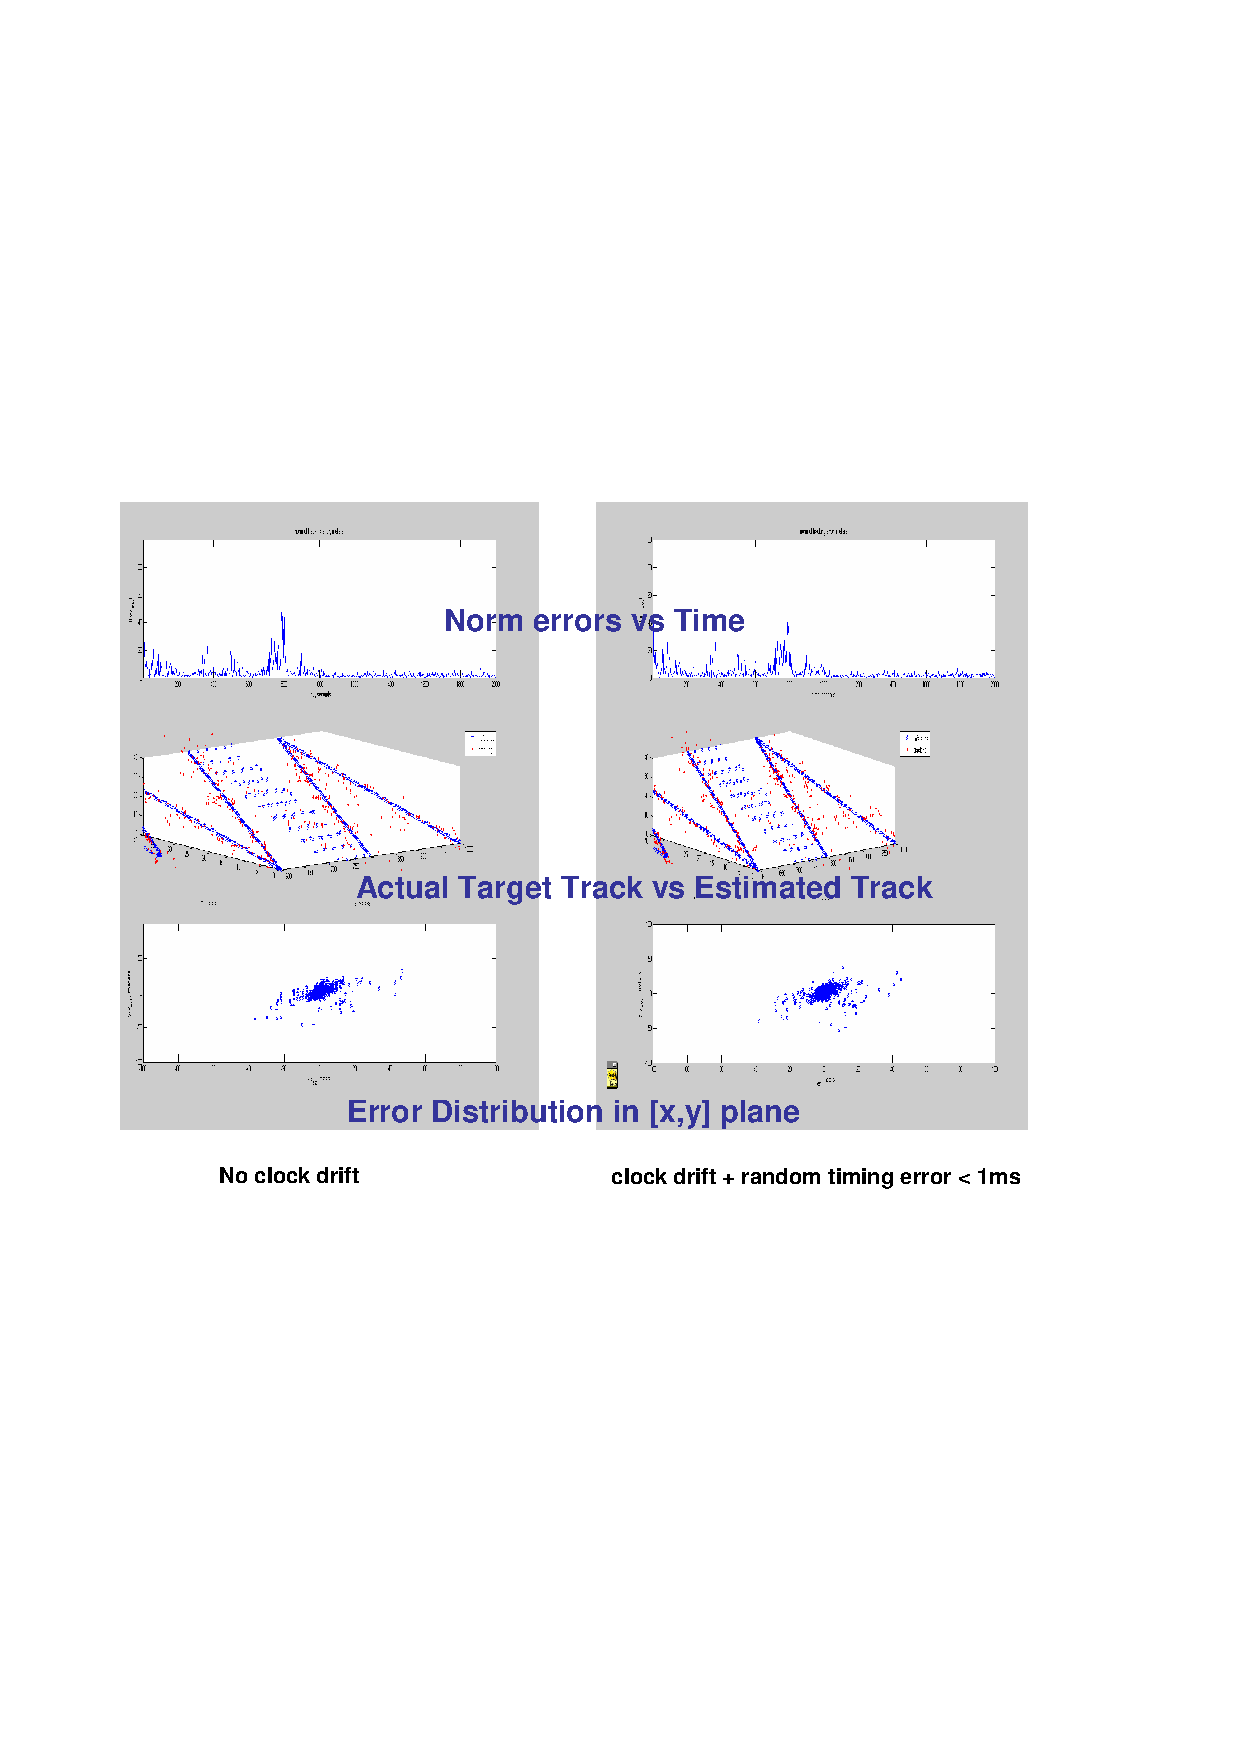
\includegraphics[height=0.45\textheight,width=0.45\textwidth,bbllx=38,bblly=254,bburx=510,bbury=605]{figures/estimationlow}
    \caption{Target Tracking in a low mobility with timing errors. 10 sensors are randomly placed in 50x50 $m^2$ field. Each sensor reports the sample to the target every 5 seconds. The target moves with speed less than 10m/s}
        \label{fig:estimation_low}
    \end{center}
\end{figure}

\begin{figure}
    \begin{center}

    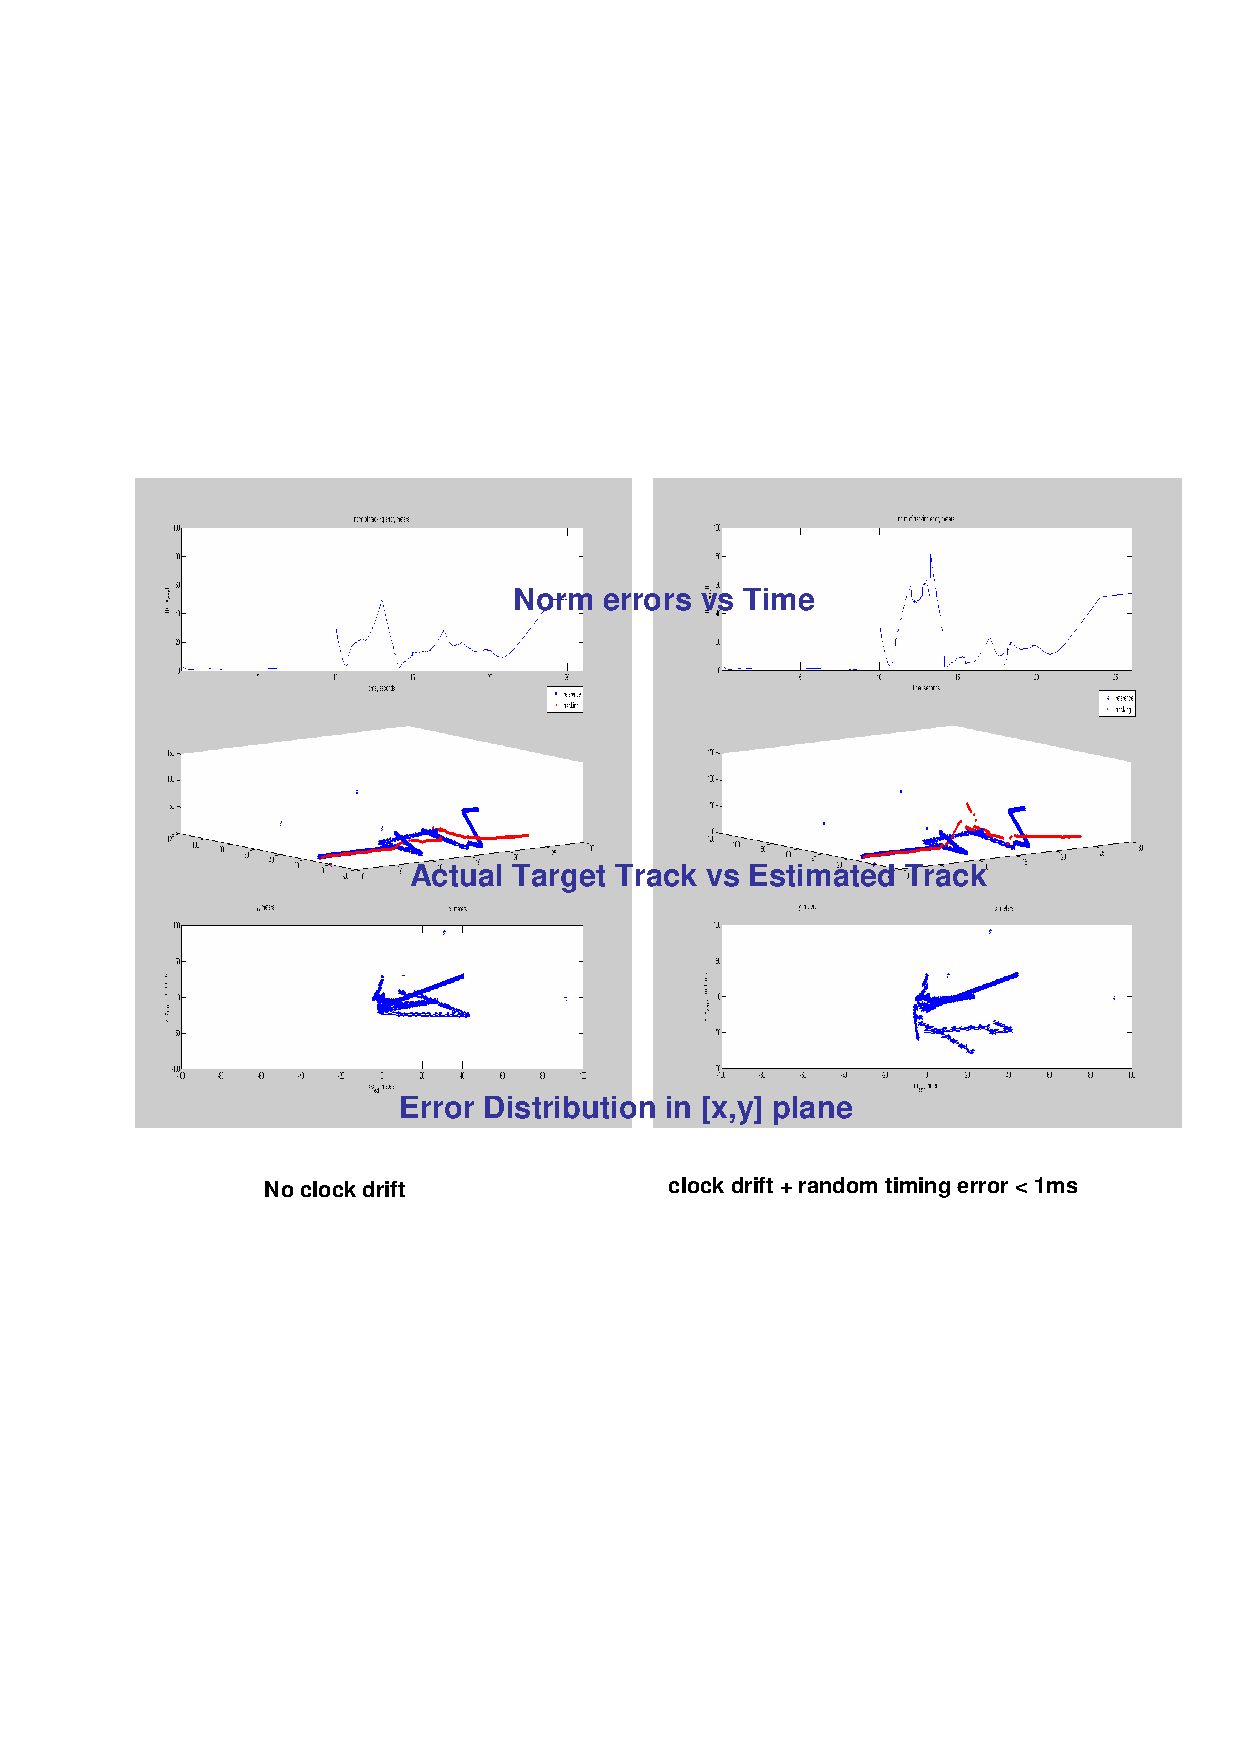
\includegraphics[height=0.45\textheight,width=0.45\textwidth,bbllx=51,bblly=262,bburx=588,bbury=615]{figures/estimationhigh}
    \caption{Target Tracking in a high mobility with timing errors. 10 sensors are randomly placed in 50x50 $m^2$ field. Each sensor reports the sample to the target every 5 seconds. The target moves with speed of 10 $\sim$ 20 m/s. }
        \label{fig:estimation_high}
    \end{center}
\end{figure}

The figures \ref{fig:estimation_low} and \ref{fig:estimation_high}
demonstrate the performance of target tracking using the proposed
filtering algorithm with or without timing errors. Each figure has
three sub-figures. First, it shows the normalized error
$\sqrt{(x'-x_t)^2+(y'-y_t)^2}$ (where $x'$ is the estimated x
location of the target, $x_t$ is the actual location x of the
target) with time. The second graph shows the actual target's
position in blue solid line and the estimated positions in (x,y)
plane in red dotted line. The last diagram shows
([$x'-x_t$,$y'-y_t$]). The results indicate that the filtering is
robust with timing errors less than 1ms. Generally, the
synchronization error through networked time synchronization
mechanisms can achieve less than a few milliseconds error. With high
mobility where target moves faster, the performance degradation with
timing error becomes noticeable. Yet, our scheme is much more robust
to timing errors compared to Least Squares mechanisms shown in
Section \ref{sec:least_square}.

\subsection{Motivation}
The motivation for the above nonlinear hybrid filter was to obtain a filter with globally stable performance (rather than the local stability obtained for an extended Kalman filter), robustness to synchronization errors, inexpensive distributable computation (unlike, for example a particle filter), and the ability to handle uncertainty in sensor location directly. Robustness is accomplished through using a filter with a minimum number of parameters--all of which have a physical significance and do not have to be chosen for specific circumstances of installation of the sensor network. through study of the filter's structure, we see that it is instantaneously unobservable, indeed, the observability matrix for the pair $\left(\mathbf{C}\left(\mathbf{x}(k)\right),\mathbf{A}\right)$ is
\begin{eqnarray}
    \mathbb{O}&=&\left(\begin{array}{c}\mathbf{C}\left(\mathbf{x}(k)\right)\\
    \mathbf{C}\left(\mathbf{x}(k)\right)\mathbf{A}\\
    \mathbf{C}\left(\mathbf{x}(k)\right)\mathbf{A}^2\\
    \mathbf{C}\left(\mathbf{x}(k)\right)\mathbf{A}^3\\
    \mathbf{C}\left(\mathbf{x}(k)\right)\mathbf{A}^4\\
    \mathbf{C}\left(\mathbf{x}(k)\right)\mathbf{A}^5\\
    \end{array}\right)\label{eqn:obsvmatrix}\\
    &=&\begin{pmatrix}
         -m_i & 0 & 0 & 1 & 0 & 0 \\
         0 & -m_i & 0 & 0 & 1 & 0 \\
         0 & 0 & -m_i & 0 & 0 & 1 \\
         0 & 0 & 0 & 0 & 0 & 0 \\
         0 & 0 & 0 & 0 & 0 & 0 \\
         0 & 0 & 0 & 0 & 0 & 0 \\
       \end{pmatrix}
    \label{eqn:obsveig},
\end{eqnarray}
with three non-zero eigenvalues $m_i^2+1$. The intuition for the working of this filter comes from Monte-Carlo methods for thresholding extreme phenomena, where there is short term divergence and long term convergence. We can be reasonably sure of being able to prove the convergence of this filter given that it's tracking error converges to zero in simulations over a wide range of sensor placement, number and tracking object speed. The tools envisioned for this are direct analysis of the sort that is performed for Kalman filters~\cite{SOLO,BOUGEROL}, Barrier certificates to show reliable performance~\cite{PRAJ,GLA}, or stochastic hybrid system tools.

\subsection{Sensitivity to Synchronization Error of Batch Least Squares over the Network}\label{sec:least_square}
This sensitivity analysis applies to least squares or any equivalent
recursive method that attains the least squares solution. We perform
the analysis for a constant velocity model of the tracked object
simply for the purpose of illustration. Suppose that the cartesian
coordinates of a moving object are given the equations
\begin{eqnarray}
x(k)&=&x_0+v_xkT\label{eqn:xconstvel}\\
y(k)&=&y_0+v_ykT\label{eqn:yconstvel},
\end{eqnarray}
then we can construct an array of sequential measurements for the least squares estimation of object position and velocity, with the object of extracting $x_0, v_x, y_0$ and $v_y$. It would have the following form:
\begin{eqnarray}
\mathbb{A}\mathbf{X}&=&\mathbb{B}\label{eqn:batchls1}\\
\mathbb{A}&=&\begin{pmatrix}
               1 & kT & -m_{k,j} &-m_{k,j}kT  \\
               1 & (k+p_1)T & -m_{k+p_1,l} & -m_{k,j}(k+p_1)T \\
               \vdots & \vdots & \vdots & \vdots \\
               1 & (k+p_n)T & -m_{k+p_n,n} & -m_{k+p_n,n}(k+p_n)T \\
             \end{pmatrix}\nonumber\\
\mathbb{B}&=&\begin{pmatrix}
               y_j-m_{k,j}x_j \\
               y_j-m_{k,j}x_j \\
               \vdots \\
               y_n-m_{k+p_n,j}x_n \\
             \end{pmatrix}\nonumber\\
\mathbf{X}&=&\begin{pmatrix}
               y_0 & v_y & x_0 & v_x \\
             \end{pmatrix}^T\nonumber,
\end{eqnarray}
where $T$ is the sample period, $j...n$ are sensor labels, $(x_j,y_j)$ is a sensor position on the plane, $m_{k,j}$ is the slope measurement from sensor $j$ at time $kT$, $k$ going from $k...k+p_n$. From the structure of this least squares problem, if we assume that there are no errors in sensor locations, the synchronization error comes additively into the matrix $\mathbb{A}$ as
\begin{eqnarray}
\mathbb{\delta A}&=&\begin{pmatrix}
               0 & a_0 & 0 &-m_{k,j}a_0 \\
               0 & a_1 & 0 & -m_{k,j}a_1 \\
               \vdots & \vdots & \vdots & \vdots \\
               0 & a_n & 0 & -m_{k+p_n,n}a_n \\
             \end{pmatrix}\label{eqn:ALSError}\\
&=&\begin{pmatrix}
               a_0 \\
               a_1 \\
               \vdots \\
               a_n \\
             \end{pmatrix}^T\begin{pmatrix}
               0 & 1 & 0 &-m_{k,j} \\
               0 & 1 & 0 & -m_{k,j} \\
               \vdots & \vdots & \vdots & \vdots \\
               0 & 1 & 0 & -m_{k+p_n,n} \\
             \end{pmatrix}\label{eqn:ALSError1}\\
&=&\begin{pmatrix}
               a_0 &
               a_1 &
               \hdots &
               a_n
             \end{pmatrix}\delta\mathbb{A'}
\end{eqnarray}
where $a_1,\ldots,a_n$ are the timing errors for the different sensors. For a least squares problem, the first order error in estimation of the unknown given the uncertainty in the regression matrix $\mathbb{A}$ is available from standard references~\cite{BJORK}:
\begin{equation}
\delta \mathbf{X}=\mathbb{A}^\dag\left(\delta \mathbb{B}-\delta\mathbb{A}\mathbf{X}\right)+\left(\mathbb{A}^T\mathbb{A}\right)^{-1}\delta\mathbb{A}^T\mathbf{r},
\end{equation}
where $\mathbf{r}=\mathbb{B}-\mathbb{A}\mathbf{X}$, and $\mathbb{A}^\dag=\left(\mathbb{A}^T\mathbb{A}\right)^{-1}\mathbb{A}^T$ is the More-Penrose inverse of $\mathbb{A}$. If we assume a mean synchronization error of $\bar{a}$ for all of the sensors, we have an estimation error that is directly proportional to it, in the form:
\begin{equation}
\delta \mathbf{X}=-\bar{a}\left(\mathbb{A}^\dag\left(\delta\mathbb{A'}\mathbf{X}\right)-\left(\mathbb{A}^T\mathbb{A}\right)^{-1}\delta\mathbb{A'}^T\mathbf{r}\right),
\end{equation}
 showing that the expected estimation error (assuming that the residual $\mathbf{r}$ is zero mean) is proportional to the product of the synchronization error and the estimate $\mathbf{X}$. Thus, faster object motion or more distant objects will increase the estimation error induced by synchronization error.

%\input{adaptation_sim}
%\input{adaptation-2}
\section{Cost-Benefit Analysis of Clock Stability and Synchronization 
on Duty Cycling, Bandwidth, and Power Consumption}
\label{sec:power}

It is generally assumed that using a more stable clock will improve the duty
cycling capabilities of an embedded system and save bandwidth since less 
frequent resynchronizations are necessary. Dutta
showed in \cite{dutta2007procrastination} that the lower bound of a clock with
a stability of $\pm 50$ppm is a duty cycle of 0.01\% for a scheduled
communication MAC protocol. But, how much additional power and bandwidth could be saved by
employing a more stable clock, considering that a more stable clock consumes
more power? The bounds on synchronization error derived in this section along 
with the constraints on power consumption are for use in designing the applications 
on the network, such as the detector in Section \ref{sec:detector}, which uses a maximum 
synchronization error as an input parameter: $\epsilon$ for the case without 
synchronization, and $b$ for the case with synchronization algorithms.


\subsection{Clock Stability and Duty Cycling}
Let us compare two systems, $A$ and $B$. Both systems have the same sleep power
consumption $P_s$ and active power consumption $P_a$.  Each node has a local
clock source with stability $s_A$ and $s_B$ (in $Hz/Hz$) that consume power $P_{cA}$ and $P_{cB}$,
respectively. Additionally, we assume that both platforms have the same duty
cycle ratio $DC$ between sleep ($T_s$) and active time ($T_a$). However, in order
to communicate with their peers, both systems include a guard time that is
proportional to their local clock source's stability $T_{gX} = 2 \cdot T_s \cdot
s_X$, where $s_X$ is the system's local clock stability. This guard time
allows the nodes to compensate for the drift in their clock while asleep by starting 
the synchronization process early enough to ensure that both nodes are awake when 
the active period starts. The guard time is set by the resynchronization period, which,
 in this case, is the sleep period since we assume nodes will resynchronize when 
they are awake.

Given these definitions, we can compute the overall power consumption of the
system and its clock in the sleep, active and guard periods as follows:
\begin{equation}
	P_X = \frac{T_s \cdot (P_s + P_{cX}) + (T_{gX} + T_a) \cdot (P_a + P_{cX})}{T_s + T_s + T_{gX}}.
\end{equation}

Where $X$ is either $A$ or $B$. Let us also assume that $s_A > s_B$ and, without loss 
of generality, that $P_{cA} < P_{cB}$. In order for system $B$ to be more efficient 
than system $A$ we have to show that
\begin{equation}
	P_A > P_B,
\end{equation}
and thus
\begin{eqnarray}
	\lefteqn{\frac{T_s \cdot (P_s + P_{cA}) + (T_{gA} + T_a) \cdot (P_a + P_{cA})}{T_s + T_a + T_{gA}}  > } \nonumber \\
	& & \frac{T_s \cdot (P_s + P_{cB}) + (T_{gB} + T_a) \cdot (P_a +
	P_{cB})}{T_s + T_a + T_{gB}}.\label{eq:1}
\end{eqnarray}

We now assume that the clock of system $A$ is an inexpensive quartz crystal as
found in many embedded systems. These crystals consume very little power, and thus
$P_{cA} \sim 0$. Using this assumption, Equation \ref{eq:1} can be simplified to
\begin{equation}
%	P_{cB} & < & \frac{T_s P_s + (T_{gA} + T_a) \cdot P_a}{T_s + T_a + T_{gA}}
%	\nonumber \\
%	& & - \frac{T_s P_s + (T_{gB} + T_a) \cdot P_a}{T_s + T_a + T_{gB}} \nonumber \\
P_{cB} < \frac{2\cdot T_s^2\cdot(P_a-P_s)\cdot(s_A-s_B)}{(T_s\cdot(1+2s_A)+T_a)(T_s\cdot(1+2s_B)+T_a)},
	\label{eq:2}
\end{equation}
where we replaced $T_{gA}$ and $T_{gB}$ with its respective definition. By definition, 
the duty cycle of the system is $DC=T_a/(T_a + T_s)$. Since clock stability is fairly low 
(usually measured in $ppm$), we can assume that $s_A, s_B << 1$. The relations are then 
simplified to
\begin{equation}
	P_{cB} < 2 \cdot [1-DC]^2\cdot (P_a-P_s) \cdot (s_A-s_B).
\end{equation}
This relation shows that for system $B$ to be more energy efficient than system $A$, 
its clock power consumption cannot exceed a threshold that depends on the duty cycle, 
the difference in active and sleep power consumption and the difference in their
clock stability. 
If we further assume that $DC << 1$, $P_s \rightarrow 0$, and $s_A >> s_B$ we find the 
relation trivially simplifies to:
\begin{equation}
	P_{cB} < 2 \cdot P_a \cdot s_A.
\end{equation}

This shows that in order for system $B$ to be more energy efficient than system
$A$, the clock system used in system $B$ has to use less power than the active
power consumption multiplied by twice the precision of system $A$'s clock
stability. For example, if we assume that $P_a=1W$, $s_A=50 ppm$, and $s_B=1
ppm$ (in order to satisfy $s_A >> s_B$) then $P_{cB} < 100 \mu W$. We
are currently unaware of any technology that can achieve a clock stability of
$1ppm$ with a power budget of less than $100 \mu W$. The closest commercially
available is the MAXIM DS32BC35 \cite{maxim2008ds32b35} which is
an RTC with integrated 32kHz TCXO, and consumes about 600mW for a stability of
$\pm 3.5ppm$. 

In this analysis, however, we have ignored the fact that time synchronization
protocols, such as FTSP \cite{maroti2004ftsp}, can estimate the current clock
drift very accurately and thus, as long as the temperature doesn't change too
quickly, can improve the duty cycling of an embedded system without using a
higher stability clock source. We conclude thus, that better clock stability 
is not always energy efficient, due to the expense of higher power in the clock
subsystem itself.  

\subsection{Bandwidth Benefits}

It is clear that a time synchronization protocol based on a less
stable clock needs to resynchronize more often, than one based on
a more stable clock. But by how much? In the simplest case,
which represents an upper bound, the time synchronization algorithm assumes
the worst case drift $s_{\max}$ and calculates the necessary resynchronization
time interval $T_r$ based on a maximum time synchronization error
$\epsilon$

\begin{equation}
    T_r < \frac{\epsilon}{s_{\max}}.
\end{equation}

This is a very conservative estimate and doesn't include the fact that a time
synchronization protocol can calculate the current clock drift. Additionally,
if we have knowledge of how fast temperature changes in the environment and
how it affects the system clock, a much better estimate of $T_r$ can be found. 

\begin{figure}
    \begin{center}
        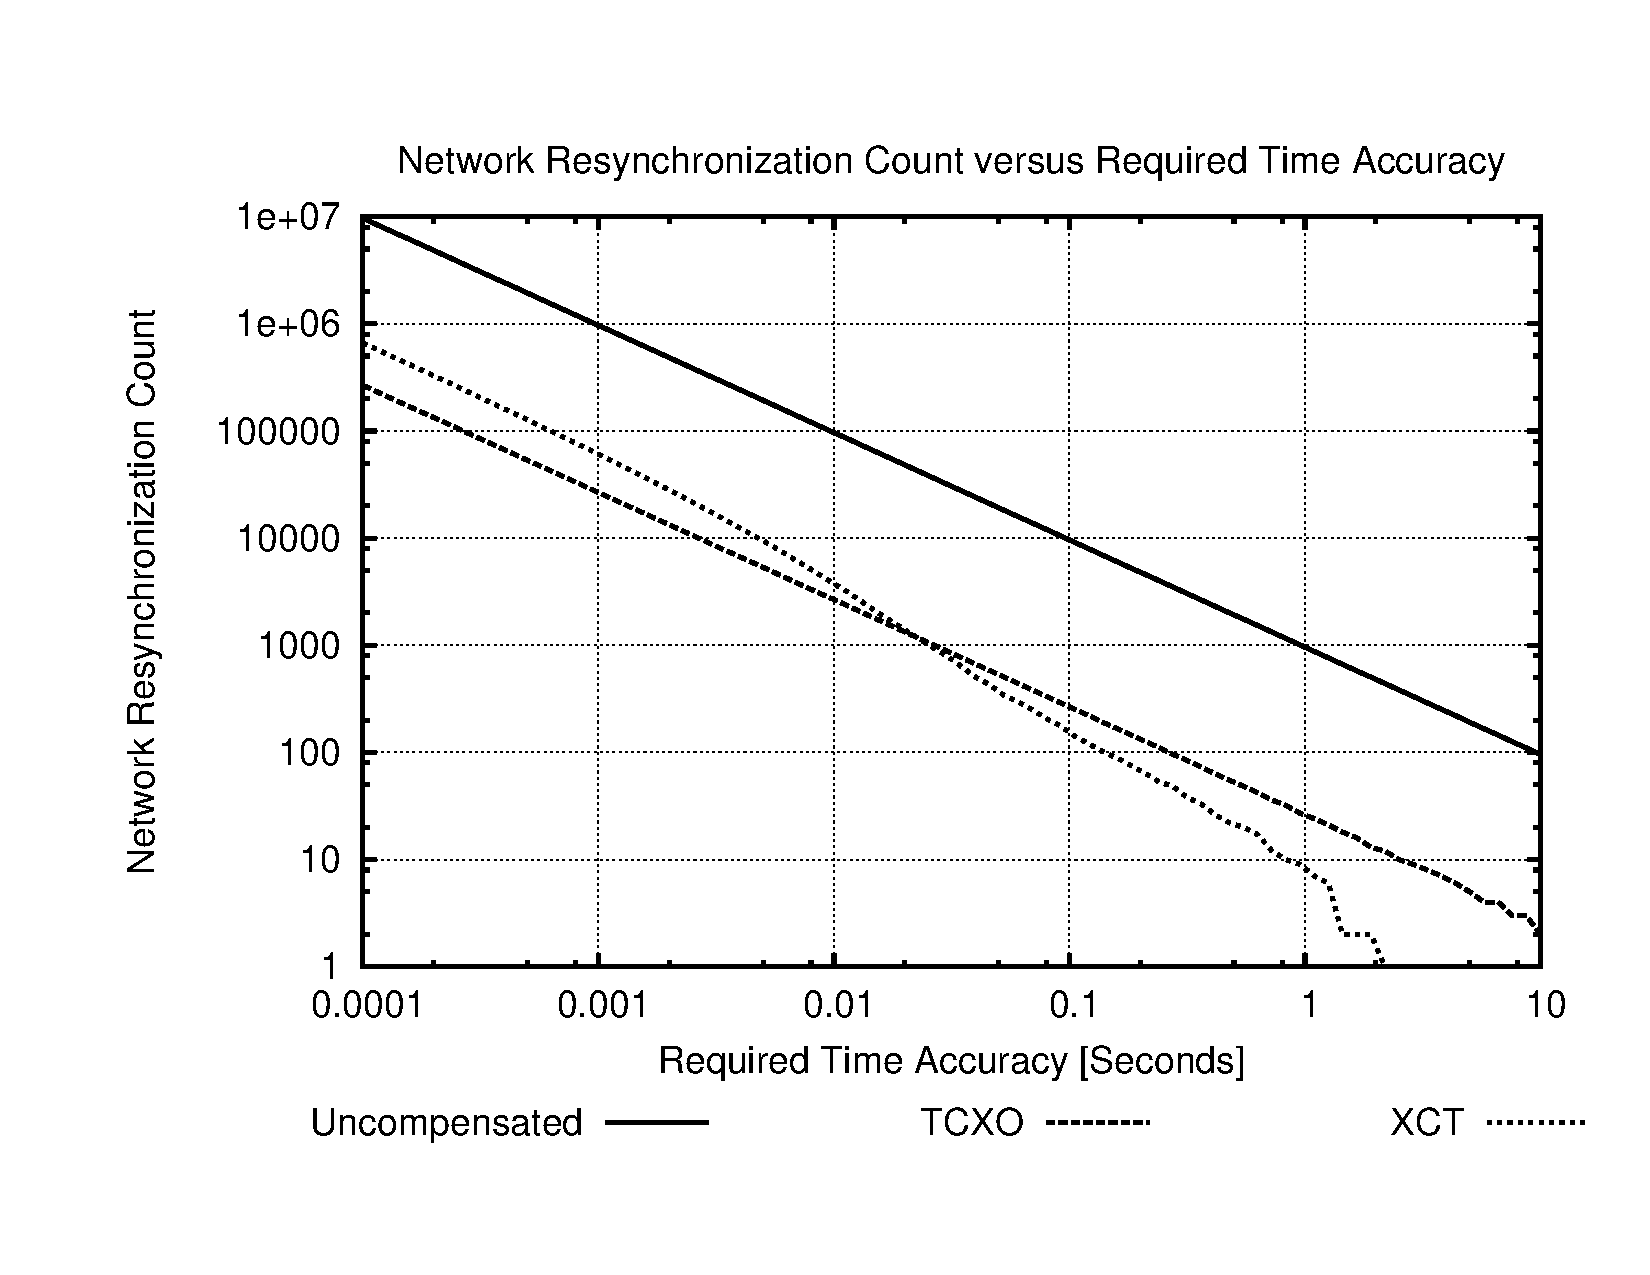
\includegraphics[angle=-90,width=0.45\textwidth]{figures/mosscamresync}
        \caption{Upper and lower bounds for the number of resynchronizations
        necessary to achieve a given time synchronization error. The
        temperature data comes from a 3 year dataset.}
        \label{fig:resync}
    \end{center}
\end{figure}

The question that arises is what would the optimal resynchronization interval be
that guarantees that synchronization error is bounded by
$\epsilon$? Assuming the system has access to an oracle that issues
the current synchronization error, and that the system does not compensate for
local clock drift, it is clear that a system with a lower drift clock will
resynchronize less often than one with a higher drift. Figure \ref{fig:resync}
illustrates this by using a 3 year temperature dataset collected at the James
Natural Wildlife Reserve \cite{mosscam}. It shows the upper and lower bounds
by calculating how often a system would have to resynchronize experiencing the
temperature changes recorded in the dataset. Looking at a specific example,
we can calculate the bandwidth savings a better clock stability can achieve.
Let's assume that the application needs a synchronization accuracy of
$\epsilon<1ms$. Over the 3 year period, an uncompensated clock would have to
resynchronize at least 900'000 times, whereas a compensated
TCXO only 25'000 times. Now, assuming that each resynchronization consists of
2 messages of 16 bytes each, results in an average bandwidth of 2.35 bit/s for
the uncompensated clock, and only 0.065 bit/s for a compensated clock.

Even though this shows that a compensated clock can lower the number of
necessary resynchronizations, it does not mean that a time synchronization
system needs to employ a TCXO to achieve this compensation. Maroti et al.
showed in \cite{maroti2004ftsp} that FTSP can estimate the current clock drift
below an accuracy of 0.1ppm. Thus, as long as the environment temperature
doesn't change too often, drift compensation can be achieved in software to a
very high accuracy.


\section{Concluding Remarks}
We have quantified the impact of network synchronization on both detection and estimation problems over sensor networks. We have also performed a cost benefit analysis of performing synchronization and clock stabilization on network nodes. Our results can be used in a twofold manner--to design the network to support these applications, and to design the applications around the constraints imposed by the network that supports them. 

\indent Our results show that network synchronization may not be necessary for certain estimation and tracking problems. In these problems, the randomness of the sensor locations combined with randomness of sense times can be used to obtain global stability and convergence of the estimation problem. The smoothing properties of estimators, including batch least squares and Kalman filters can be used to naturally reduce overall tracking error.

\indent For detection problems, our analysis shows that synchronization becomes important when the events detected are of short duration and frequent. It is also needed when the parameters of an event, such as the location and intensity of an explosion need to be estimated in real-time. Our analysis of the detection combined with the cost-benefit analysis of synchronization provides immediate solutions to setting detection thresholds and to the choice of synchronization scheme and frequency, along with clock accuracy needed. 
\section*{Acknowledgements}
We would like to thank Dr. Srivatsan Varadarajan for discussions on problem formulation in the detection problem and Dr. Vic Thomas for discussions on the actual application of the tracking filter. 
\bibliography{ref}
\bibliographystyle{plain}

\end{document}
